\paragraph{POST /:lang/recovery}
\begin{itemize}
\item \textbf{Successo}
Quando un utente registrato dimentica la propria password ha la possibilità di accedere al proprio account facendosi inviare una nuova password nell'indirizzo email utilizzato durante la registrazione. Questo scenario rappresenta il successo di una procedura di \textit{recovery} per password dimenticata con vincolo che l'utente sia registrato, ma non autenticato. Il sistema dovrà occuparsi di generare un password, inviarla all'indirizzo email dell'utente e di cambiarla nel suo rispettivo account.

\label{Procedura di recupero password}
\begin{figure}[ht]
	\centering
	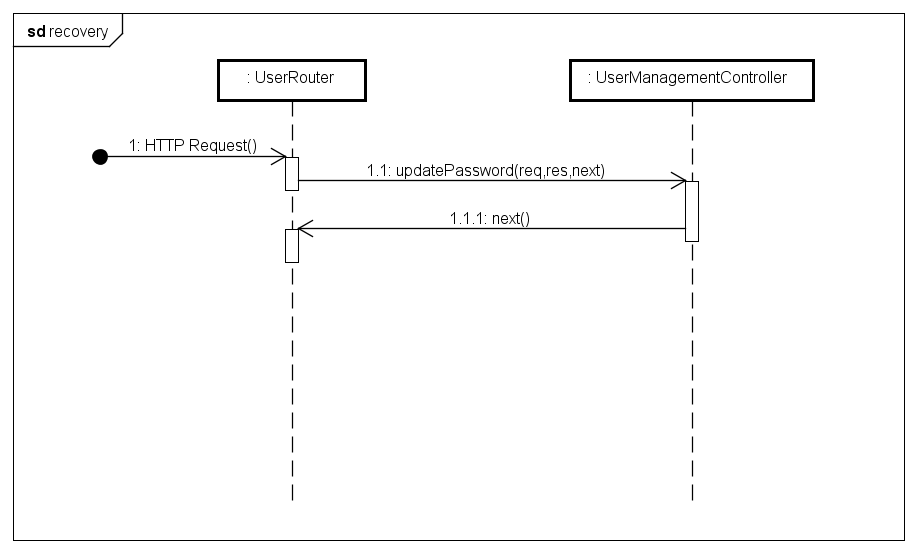
\includegraphics[scale=0.40]{UML/DiagrammiDiSequenza/Back-end/POST__lang_recovery_success.png}
	\caption{POST /:lang/recovery}
\end{figure}
\FloatBarrier

\item \textbf{Fallimento}
Quando un utente richiede un recupero della password inserendo una email non presente nel sistema, viene sollevato un errore. Tale scenario rappresenta il fallimento di una richiesta di recupero della password che impone, come vincolo per poter essere effettuata, che l'utente non sia autenticato. In questo caso il modulo \texttt{AuthenticationController} invia \texttt{next(error)} per il fallimento di tale vincolo al router, il quale avrà compito di reinstradarlo (indirizzandolo verso \texttt{ErrorHandler}).

\label{Fallimento procedura di recupero password}
\begin{figure}[ht]
	\centering
	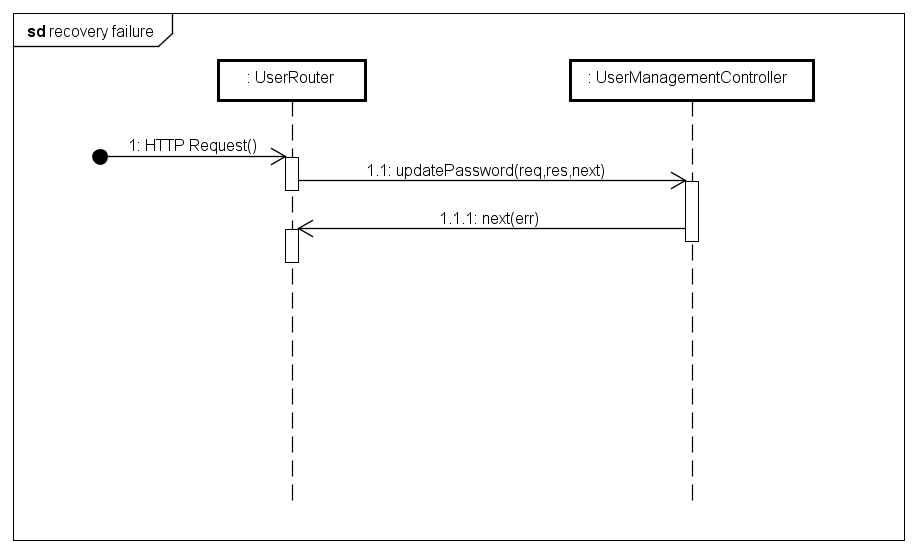
\includegraphics[scale=0.40]{UML/DiagrammiDiSequenza/Back-end/POST__lang_recovery_failure.png}
	\caption{Fallimento della procedura di recupero della password}
\end{figure}
\FloatBarrier

\end{itemize}